% This file was created by tikzplotlib v0.9.1.
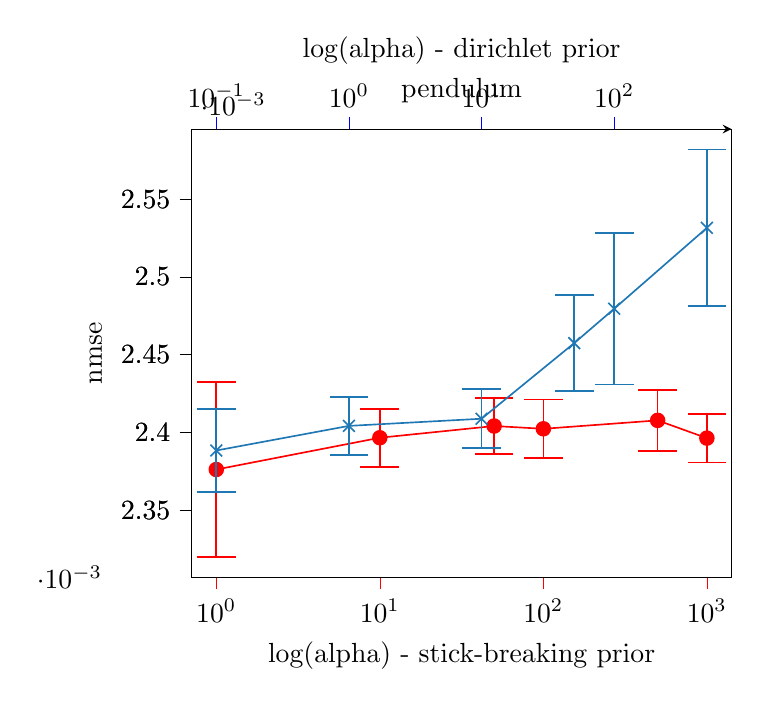
\begin{tikzpicture}

\definecolor{color0}{rgb}{0.12156862745098,0.466666666666667,0.705882352941177}

\begin{axis}[
log basis x={10},
tick align=outside,
tick pos=left,
title={pendulum},
x grid style={white!69.0196078431373!black},
xlabel={log(alpha) - stick-breaking prior},
xmin=0.707945784384138, xmax=1412.53754462275,
xmode=log,
xtick style={color=red},
xtick={0.01,0.1,1,10,100,1000,10000,100000},
xticklabels={\(\displaystyle {10^{-2}}\),\(\displaystyle {10^{-1}}\),\(\displaystyle {10^{0}}\),\(\displaystyle {10^{1}}\),\(\displaystyle {10^{2}}\),\(\displaystyle {10^{3}}\),\(\displaystyle {10^{4}}\),\(\displaystyle {10^{5}}\)},
y grid style={white!69.0196078431373!black},
ylabel={nmse},
ymin=0.0023068208357579, ymax=0.00259501543045457,
ytick style={color=black}
]
\path [draw=red, semithick]
(axis cs:1,0.00231992059006229)
--(axis cs:1,0.00243240255955748);

\path [draw=red, semithick]
(axis cs:10,0.00237792218918827)
--(axis cs:10,0.00241525543997751);

\path [draw=red, semithick]
(axis cs:50,0.00238613603717064)
--(axis cs:50,0.00242211021451883);

\path [draw=red, semithick]
(axis cs:100,0.0023835379740462)
--(axis cs:100,0.00242114247532584);

\path [draw=red, semithick]
(axis cs:500,0.00238824944151183)
--(axis cs:500,0.00242724022342822);

\path [draw=red, semithick]
(axis cs:1000,0.00238062391328215)
--(axis cs:1000,0.00241205266002244);

\addplot [semithick, red, mark=-, mark size=7, mark options={solid}, only marks]
table {%
1 0.00231992059006229
10 0.00237792218918827
50 0.00238613603717064
100 0.0023835379740462
500 0.00238824944151183
1000 0.00238062391328215
};
\addplot [semithick, red, mark=-, mark size=7, mark options={solid}, only marks]
table {%
1 0.00243240255955748
10 0.00241525543997751
50 0.00242211021451883
100 0.00242114247532584
500 0.00242724022342822
1000 0.00241205266002244
};
\addplot [semithick, red, mark=*, mark size=2.5, mark options={solid}]
table {%
1 0.00237616157480988
10 0.00239658881458289
50 0.00240412312584473
100 0.00240234022468602
500 0.00240774483247002
1000 0.00239633828665229
};
\end{axis}

\begin{axis}[
axis x line=top,
log basis x={10},
tick align=outside,
x grid style={white!69.0196078431373!black},
xlabel={log(alpha) - dirichlet prior},
xmin=0.0653208007180445, xmax=765.452956031933,
xmode=log,
xtick pos=right,
xtick style={color=blue},
xtick={0.001,0.01,0.1,1,10,100,1000,10000},
xticklabels={\(\displaystyle {10^{-3}}\),\(\displaystyle {10^{-2}}\),\(\displaystyle {10^{-1}}\),\(\displaystyle {10^{0}}\),\(\displaystyle {10^{1}}\),\(\displaystyle {10^{2}}\),\(\displaystyle {10^{3}}\),\(\displaystyle {10^{4}}\)},
y grid style={white!69.0196078431373!black},
ymin=0.0023068208357579, ymax=0.00259501543045457,
ytick pos=left,
ytick style={color=black}
]
\path [draw=color0, semithick]
(axis cs:0.1,0.00236176092856157)
--(axis cs:0.1,0.00241501442172194);

\path [draw=color0, semithick]
(axis cs:1,0.00238557317995135)
--(axis cs:1,0.00242284523186021);

\path [draw=color0, semithick]
(axis cs:10,0.0023898435870136)
--(axis cs:10,0.0024277729224975);

\path [draw=color0, semithick]
(axis cs:50,0.00242644444513833)
--(axis cs:50,0.00248843502568972);

\path [draw=color0, semithick]
(axis cs:100,0.00243086295080997)
--(axis cs:100,0.0025281712595606);

\path [draw=color0, semithick]
(axis cs:500,0.00248111921592768)
--(axis cs:500,0.00258191567615017);

\addplot [semithick, color0, mark=-, mark size=7, mark options={solid}, only marks]
table {%
0.1 0.00236176092856157
1 0.00238557317995135
10 0.0023898435870136
50 0.00242644444513833
100 0.00243086295080997
500 0.00248111921592768
};
\addplot [semithick, color0, mark=-, mark size=7, mark options={solid}, only marks]
table {%
0.1 0.00241501442172194
1 0.00242284523186021
10 0.0024277729224975
50 0.00248843502568972
100 0.0025281712595606
500 0.00258191567615017
};
\addplot [semithick, color0, mark=x, mark size=3, mark options={solid}]
table {%
0.1 0.00238838767514175
1 0.00240420920590578
10 0.00240880825475555
50 0.00245743973541402
100 0.00247951710518529
500 0.00253151744603893
};
\end{axis}

\end{tikzpicture}
